% Diagrams for the SVD page. Each tikzpicture becomes one SVG.
%
% Build (from this folder):
%   latex diagrams.tex
%   dvisvgm --no-fonts --exact-bbox --page=1- --output=fig-%p diagrams.dvi
%   mv fig-1.svg svd_matrix.svg
%   mv fig-2.svg svd_truncated.svg
%   mv fig-3.svg svd_diagram.svg
%   mv fig-4.svg svd_isometry.svg
%   mv fig-5.svg svd_tensor.svg
%   rm -f diagrams.aux diagrams.log diagrams.dvi
%
% Colors and line weights follow the other figures on the site
% (see also mps/algorithms/ttsvd/diagrams.tex):
% gray = generic tensor, pink = U, blue = singular values, orange = V^dagger.

\documentclass[dvisvgm,tikz,border=4pt]{standalone}
\usepackage{newtxtext,newtxmath}
\usetikzlibrary{calc}

\definecolor{tgray}{HTML}{D5D5D5}
\definecolor{tpink}{HTML}{CB6D9D}
\definecolor{tblue}{HTML}{82A2DA}
\definecolor{torange}{HTML}{FFA902}

\tikzset{
  every picture/.style={line width=1.6pt, line cap=butt},
  sq/.style={draw, line width=1.6pt, minimum size=0.62cm, inner sep=0pt},
  gen/.style={sq, fill=tgray},
  iso/.style={sq, fill=tpink},
  vdag/.style={sq, fill=torange},
  sv/.style={draw, line width=1.6pt, circle, fill=tblue, minimum size=0.48cm, inner sep=0pt},
  pill/.style={draw, line width=1.6pt, fill=tgray, rounded corners=5pt,
               minimum height=0.62cm, inner sep=0pt},
  lbl/.style={font=\large},
  idx/.style={font=\normalsize},
  dim/.style={font=\normalsize},
  op/.style={font=\LARGE},
  % matrix cartoons
  matbox/.style={line width=1.6pt},
  ghost/.style={line width=1.0pt, draw=black!45, dash pattern=on 3pt off 2pt, fill=white},
  entry/.style={line width=0.9pt},
}

% size of one matrix entry in the cartoons
\def\c{0.36}

% \legs{node}{n}: n evenly spaced legs on top of a node
\newcommand{\legs}[2]{%
  \foreach \j in {1,...,#2} {
    \draw ($(#1.north west)!{(\j-0.5)/#2}!(#1.north east)$) -- ++(0,0.5);
  }%
}

% \matrect[style]{x}{y}{rows}{cols}: rectangle with top-left corner (x,y)
\newcommand{\matrect}[5][]{%
  \draw[matbox, #1] (#2,#3) rectangle ++(#5*\c,-#4*\c);
}

\begin{document}

% ------------------------------------------------------------------
% 1. Cartoon of the (thin) SVD of a 6 x 4 matrix
% ------------------------------------------------------------------
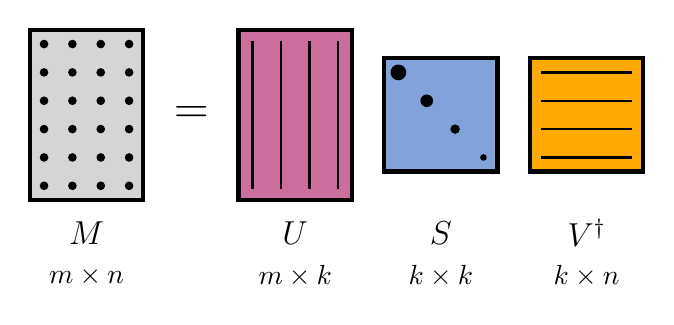
\begin{tikzpicture}
  % M: 6 x 4 matrix of generic entries
  \matrect[fill=tgray]{0}{1.08}{6}{4}
  \foreach \i in {1,...,6} \foreach \j in {1,...,4}
    \fill ({(\j-0.5)*\c},{1.08-(\i-0.5)*\c}) circle (0.055);
  \node[lbl] at (0.72,-1.5) {$M$};
  \node[dim] at (0.72,-2.05) {$m \times n$};

  \node[op] at (2.05,0) {$=$};

  % U: 6 x 4, orthonormal columns
  \matrect[fill=tpink]{2.65}{1.08}{6}{4}
  \foreach \j in {1,...,4}
    \draw[entry] ({2.65+(\j-0.5)*\c},{1.08-0.14}) -- ++(0,{-6*\c+0.28});
  \node[lbl] at (3.37,-1.5) {$U$};
  \node[dim] at (3.37,-2.05) {$m \times k$};

  % S: 4 x 4 diagonal, entries shrinking along the diagonal
  \matrect[fill=tblue]{4.5}{0.72}{4}{4}
  \foreach \j/\r in {1/0.10, 2/0.08, 3/0.06, 4/0.042}
    \fill ({4.5+(\j-0.5)*\c},{0.72-(\j-0.5)*\c}) circle (\r);
  \node[lbl] at (5.22,-1.5) {$S$};
  \node[dim] at (5.22,-2.05) {$k \times k$};

  % V^dagger: 4 x 4, orthonormal rows
  \matrect[fill=torange]{6.35}{0.72}{4}{4}
  \foreach \i in {1,...,4}
    \draw[entry] ({6.35+0.14},{0.72-(\i-0.5)*\c}) -- ++({4*\c-0.28},0);
  \node[lbl] at (7.07,-1.5) {$V^\dagger$};
  \node[dim] at (7.07,-2.05) {$k \times n$};
\end{tikzpicture}

% ------------------------------------------------------------------
% 2. Truncated SVD: keep the r = 2 largest singular values
% ------------------------------------------------------------------
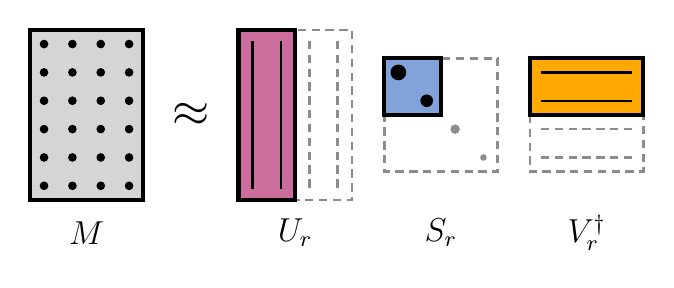
\begin{tikzpicture}
  \matrect[fill=tgray]{0}{1.08}{6}{4}
  \foreach \i in {1,...,6} \foreach \j in {1,...,4}
    \fill ({(\j-0.5)*\c},{1.08-(\i-0.5)*\c}) circle (0.055);
  \node[lbl] at (0.72,-1.5) {$M$};

  \node[op] at (2.05,0) {$\approx$};

  % U: first two columns kept, last two discarded
  \draw[ghost] ({2.65+2*\c},1.08) rectangle ++({2*\c},{-6*\c});
  \foreach \j in {3,4}
    \draw[ghost, fill=none] ({2.65+(\j-0.5)*\c},{1.08-0.14}) -- ++(0,{-6*\c+0.28});
  \matrect[fill=tpink]{2.65}{1.08}{6}{2}
  \foreach \j in {1,2}
    \draw[entry] ({2.65+(\j-0.5)*\c},{1.08-0.14}) -- ++(0,{-6*\c+0.28});
  \node[lbl] at (3.37,-1.5) {$U_r$};

  % S: top-left 2 x 2 block kept
  \draw[ghost] (4.5,0.72) rectangle ++({4*\c},{-4*\c});
  \foreach \j/\r in {3/0.06, 4/0.042}
    \fill[black!45] ({4.5+(\j-0.5)*\c},{0.72-(\j-0.5)*\c}) circle (\r);
  \matrect[fill=tblue]{4.5}{0.72}{2}{2}
  \foreach \j/\r in {1/0.10, 2/0.08}
    \fill ({4.5+(\j-0.5)*\c},{0.72-(\j-0.5)*\c}) circle (\r);
  \node[lbl] at (5.22,-1.5) {$S_r$};

  % V^dagger: first two rows kept
  \draw[ghost] (6.35,{0.72-2*\c}) rectangle ++({4*\c},{-2*\c});
  \foreach \i in {3,4}
    \draw[ghost, fill=none] ({6.35+0.14},{0.72-(\i-0.5)*\c}) -- ++({4*\c-0.28},0);
  \matrect[fill=torange]{6.35}{0.72}{2}{4}
  \foreach \i in {1,2}
    \draw[entry] ({6.35+0.14},{0.72-(\i-0.5)*\c}) -- ++({4*\c-0.28},0);
  \node[lbl] at (7.07,-1.5) {$V_r^\dagger$};
\end{tikzpicture}

% ------------------------------------------------------------------
% 3. SVD in tensor diagram notation
% ------------------------------------------------------------------
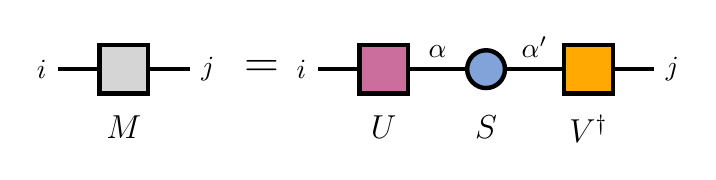
\begin{tikzpicture}
  \node[gen] (M) at (0,0) {};
  \draw (M.west) -- ++(-0.5,0) node[idx, left] {$i$};
  \draw (M.east) -- ++(0.5,0) node[idx, right] {$j$};
  \node[lbl, below=3pt] at (M.south) {$M$};

  \node[op] at (1.75,0) {$=$};

  \node[iso] (U) at (3.3,0) {};
  \node[sv] (S) at (4.6,0) {};
  \node[vdag] (V) at (5.9,0) {};
  \draw (U.west) -- ++(-0.5,0) node[idx, left] {$i$};
  \draw (U.east) -- (S.west);
  \draw (S.east) -- (V.west);
  \draw (V.east) -- ++(0.5,0) node[idx, right] {$j$};
  \node[idx, above] at ($(U.east)!0.5!(S.west)$) {$\alpha$};
  \node[idx, above] at ($(S.east)!0.5!(V.west)$) {$\alpha'$};
  \node[lbl, below=3pt] at (U.south) {$U$};
  \node[lbl, below=3pt] at (S.south |- U.south) {$S$};
  \node[lbl, below=3pt] at (V.south) {$V^\dagger$};
\end{tikzpicture}

% ------------------------------------------------------------------
% 4. U and V have orthonormal columns
% ------------------------------------------------------------------
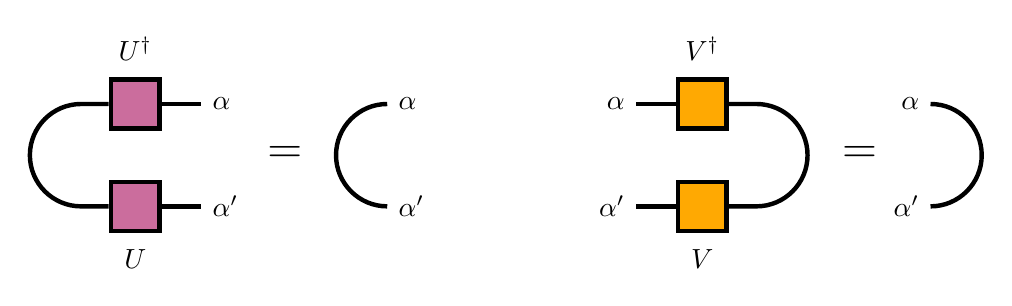
\begin{tikzpicture}
  % U^dagger U = I : contract the row index i on the left
  \node[iso] (A) at (0,0.65) {};
  \node[iso] (B) at (0,-0.65) {};
  \draw (A.west) -- ++(-0.35,0) arc[start angle=90, end angle=270, radius=0.65] -- (B.west);
  \draw (A.east) -- ++(0.5,0) node[idx, right] {$\alpha$};
  \draw (B.east) -- ++(0.5,0) node[idx, right] {$\alpha'$};
  \node[idx, above=2pt] at (A.north) {$U^\dagger$};
  \node[idx, below=2pt] at (B.south) {$U$};

  \node[op] at (1.9,0) {$=$};

  \draw (3.2,0.65) arc[start angle=90, end angle=270, radius=0.65];
  \node[idx, right] at (3.2,0.65) {$\alpha$};
  \node[idx, right] at (3.2,-0.65) {$\alpha'$};

  % V^dagger V = I : contract the column index j on the right
  \begin{scope}[xshift=7.2cm]
    \node[vdag] (C) at (0,0.65) {};
    \node[vdag] (D) at (0,-0.65) {};
    \draw (C.east) -- ++(0.35,0) arc[start angle=90, end angle=-90, radius=0.65] -- (D.east);
    \draw (C.west) -- ++(-0.5,0) node[idx, left] {$\alpha$};
    \draw (D.west) -- ++(-0.5,0) node[idx, left] {$\alpha'$};
    \node[idx, above=2pt] at (C.north) {$V^\dagger$};
    \node[idx, below=2pt] at (D.south) {$V$};

    \node[op] at (2.0,0) {$=$};

    \draw (2.9,0.65) arc[start angle=90, end angle=-90, radius=0.65];
    \node[idx, left] at (2.9,0.65) {$\alpha$};
    \node[idx, left] at (2.9,-0.65) {$\alpha'$};
  \end{scope}
\end{tikzpicture}

% ------------------------------------------------------------------
% 5. SVD of a tensor, grouping indices into two sets
% ------------------------------------------------------------------
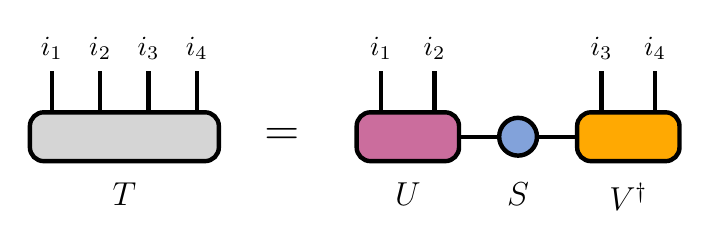
\begin{tikzpicture}
  \node[pill, minimum width=2.4cm] (T) at (0,0) {};
  \legs{T}{4}
  \foreach \j/\s in {1/i_1, 2/i_2, 3/i_3, 4/i_4} {
    \node[idx, above] at ($(T.north west)!{(\j-0.5)/4}!(T.north east)+(0,0.5)$) {$\s$};
  }
  \node[lbl, below=3pt] at (T.south) {$T$};

  \node[op] at (2.0,0) {$=$};

  \node[pill, minimum width=1.3cm, fill=tpink] (U) at (3.6,0) {};
  \legs{U}{2}
  \foreach \j/\s in {1/i_1, 2/i_2} {
    \node[idx, above] at ($(U.north west)!{(\j-0.5)/2}!(U.north east)+(0,0.5)$) {$\s$};
  }
  \node[sv] (S) at (5.0,0) {};
  \node[pill, minimum width=1.3cm, fill=torange] (V) at (6.4,0) {};
  \legs{V}{2}
  \foreach \j/\s in {1/i_3, 2/i_4} {
    \node[idx, above] at ($(V.north west)!{(\j-0.5)/2}!(V.north east)+(0,0.5)$) {$\s$};
  }
  \draw (U.east) -- (S.west);
  \draw (S.east) -- (V.west);
  \node[lbl, below=3pt] at (U.south) {$U$};
  \node[lbl, below=3pt] at (S.south |- U.south) {$S$};
  \node[lbl, below=3pt] at (V.south) {$V^\dagger$};
\end{tikzpicture}

\end{document}
